\documentclass{article}
\usepackage{tikz}

\begin{document}

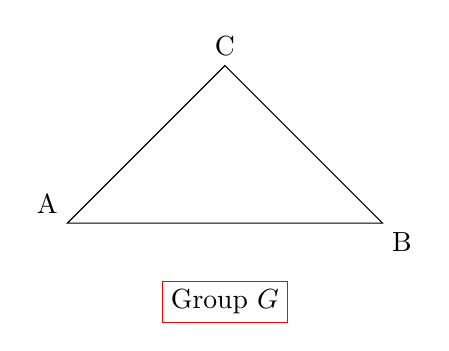
\begin{tikzpicture}[scale=2]
    % Define the coordinates for the vertices of the triangle
    \coordinate (A) at (-1, 0);
    \coordinate (B) at (1, 0);
    \coordinate (C) at (0, 1);

    % Draw the triangle
    \draw[black] (A) -- (B) -- (C) -- cycle;

    % Add labels to the vertices
    \node[above left] at (A) {A};
    \node[below right] at (B) {B};
    \node[above] at (C) {C};

    % Optionally, add some text inside the triangle
    \node[inner sep=3pt, draw=red, fill=white] at (0, -0.5) {Group $G$};
\end{tikzpicture}

\end{document}